\documentclass[]{article}
\usepackage{lmodern}
\usepackage{amssymb,amsmath}
\usepackage{ifxetex,ifluatex}
\usepackage{fixltx2e} % provides \textsubscript
\ifnum 0\ifxetex 1\fi\ifluatex 1\fi=0 % if pdftex
  \usepackage[T1]{fontenc}
  \usepackage[utf8]{inputenc}
\else % if luatex or xelatex
  \ifxetex
    \usepackage{mathspec}
    \usepackage{xltxtra,xunicode}
  \else
    \usepackage{fontspec}
  \fi
  \defaultfontfeatures{Mapping=tex-text,Scale=MatchLowercase}
  \newcommand{\euro}{€}
\fi
% use upquote if available, for straight quotes in verbatim environments
\IfFileExists{upquote.sty}{\usepackage{upquote}}{}
% use microtype if available
\IfFileExists{microtype.sty}{%
\usepackage{microtype}
\UseMicrotypeSet[protrusion]{basicmath} % disable protrusion for tt fonts
}{}
\ifxetex
  \usepackage[setpagesize=false, % page size defined by xetex
              unicode=false, % unicode breaks when used with xetex
              xetex]{hyperref}
\else
  \usepackage[unicode=true]{hyperref}
\fi
\hypersetup{breaklinks=true,
            bookmarks=true,
            pdfauthor={},
            pdftitle={},
            colorlinks=true,
            citecolor=blue,
            urlcolor=blue,
            linkcolor=magenta,
            pdfborder={0 0 0}}
\urlstyle{same}  % don't use monospace font for urls
\usepackage{color}
\usepackage{fancyvrb}
\newcommand{\VerbBar}{|}
\newcommand{\VERB}{\Verb[commandchars=\\\{\}]}
\DefineVerbatimEnvironment{Highlighting}{Verbatim}{commandchars=\\\{\}}
% Add ',fontsize=\small' for more characters per line
\newenvironment{Shaded}{}{}
\newcommand{\KeywordTok}[1]{\textcolor[rgb]{0.00,0.44,0.13}{\textbf{{#1}}}}
\newcommand{\DataTypeTok}[1]{\textcolor[rgb]{0.56,0.13,0.00}{{#1}}}
\newcommand{\DecValTok}[1]{\textcolor[rgb]{0.25,0.63,0.44}{{#1}}}
\newcommand{\BaseNTok}[1]{\textcolor[rgb]{0.25,0.63,0.44}{{#1}}}
\newcommand{\FloatTok}[1]{\textcolor[rgb]{0.25,0.63,0.44}{{#1}}}
\newcommand{\ConstantTok}[1]{\textcolor[rgb]{0.53,0.00,0.00}{{#1}}}
\newcommand{\CharTok}[1]{\textcolor[rgb]{0.25,0.44,0.63}{{#1}}}
\newcommand{\SpecialCharTok}[1]{\textcolor[rgb]{0.25,0.44,0.63}{{#1}}}
\newcommand{\StringTok}[1]{\textcolor[rgb]{0.25,0.44,0.63}{{#1}}}
\newcommand{\VerbatimStringTok}[1]{\textcolor[rgb]{0.25,0.44,0.63}{{#1}}}
\newcommand{\SpecialStringTok}[1]{\textcolor[rgb]{0.73,0.40,0.53}{{#1}}}
\newcommand{\ImportTok}[1]{{#1}}
\newcommand{\CommentTok}[1]{\textcolor[rgb]{0.38,0.63,0.69}{\textit{{#1}}}}
\newcommand{\DocumentationTok}[1]{\textcolor[rgb]{0.73,0.13,0.13}{\textit{{#1}}}}
\newcommand{\AnnotationTok}[1]{\textcolor[rgb]{0.38,0.63,0.69}{\textbf{\textit{{#1}}}}}
\newcommand{\CommentVarTok}[1]{\textcolor[rgb]{0.38,0.63,0.69}{\textbf{\textit{{#1}}}}}
\newcommand{\OtherTok}[1]{\textcolor[rgb]{0.00,0.44,0.13}{{#1}}}
\newcommand{\FunctionTok}[1]{\textcolor[rgb]{0.02,0.16,0.49}{{#1}}}
\newcommand{\VariableTok}[1]{\textcolor[rgb]{0.10,0.09,0.49}{{#1}}}
\newcommand{\ControlFlowTok}[1]{\textcolor[rgb]{0.00,0.44,0.13}{\textbf{{#1}}}}
\newcommand{\OperatorTok}[1]{\textcolor[rgb]{0.40,0.40,0.40}{{#1}}}
\newcommand{\BuiltInTok}[1]{{#1}}
\newcommand{\ExtensionTok}[1]{{#1}}
\newcommand{\PreprocessorTok}[1]{\textcolor[rgb]{0.74,0.48,0.00}{{#1}}}
\newcommand{\AttributeTok}[1]{\textcolor[rgb]{0.49,0.56,0.16}{{#1}}}
\newcommand{\RegionMarkerTok}[1]{{#1}}
\newcommand{\InformationTok}[1]{\textcolor[rgb]{0.38,0.63,0.69}{\textbf{\textit{{#1}}}}}
\newcommand{\WarningTok}[1]{\textcolor[rgb]{0.38,0.63,0.69}{\textbf{\textit{{#1}}}}}
\newcommand{\AlertTok}[1]{\textcolor[rgb]{1.00,0.00,0.00}{\textbf{{#1}}}}
\newcommand{\ErrorTok}[1]{\textcolor[rgb]{1.00,0.00,0.00}{\textbf{{#1}}}}
\newcommand{\NormalTok}[1]{{#1}}
\usepackage{graphicx,grffile}
\makeatletter
\def\maxwidth{\ifdim\Gin@nat@width>\linewidth\linewidth\else\Gin@nat@width\fi}
\def\maxheight{\ifdim\Gin@nat@height>\textheight\textheight\else\Gin@nat@height\fi}
\makeatother
% Scale images if necessary, so that they will not overflow the page
% margins by default, and it is still possible to overwrite the defaults
% using explicit options in \includegraphics[width, height, ...]{}
\setkeys{Gin}{width=\maxwidth,height=\maxheight,keepaspectratio}
\setlength{\parindent}{0pt}
\setlength{\parskip}{6pt plus 2pt minus 1pt}
\setlength{\emergencystretch}{3em}  % prevent overfull lines
\providecommand{\tightlist}{%
  \setlength{\itemsep}{0pt}\setlength{\parskip}{0pt}}
\setcounter{secnumdepth}{0}

\date{}

% Redefines (sub)paragraphs to behave more like sections
\ifx\paragraph\undefined\else
\let\oldparagraph\paragraph
\renewcommand{\paragraph}[1]{\oldparagraph{#1}\mbox{}}
\fi
\ifx\subparagraph\undefined\else
\let\oldsubparagraph\subparagraph
\renewcommand{\subparagraph}[1]{\oldsubparagraph{#1}\mbox{}}
\fi

\begin{document}
	\title{\huge\textbf{Moments}\LARGE \\Project: Marker-based Localization}
	\author{Niharika Jayanthi, Dheeraj Kamath \\Mentor: Sanam Shakya}
	\maketitle
	\pagebreak
\section{Goals}\label{goals}

\begin{itemize}
\tightlist
\item
  To understand what are moments in image processing.
\item
  To learn about Hu moments.
\item
  To use the cv2.moments(), cv2.HuMoments() functions in python.
\end{itemize}

\section{Theory}\label{theory}

\subsection{Working Principle}\label{working-principle}

\textbf{Introduction}

Moments, in image processing, are weighted average of the image pixels'
intensities. Weighted average is similar to normal average except some
values from the set contribute more to the result than the others. The
formula for spatial moments in a raster image is-

\begin{figure}[htbp]
\centering
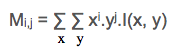
\includegraphics{images/Moments/Spatial moments.png}
\caption{Spatial Moments}
\end{figure}

Here, I(x,y) can have a value of either 0(background) or 1(foreground).

Using moments, one can obtain several properties of an image such as -

\begin{itemize}
\tightlist
\item
  \textbf{Area} :
\end{itemize}

\begin{figure}[htbp]
\centering
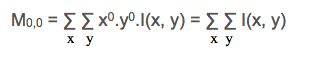
\includegraphics{images/Moments/Area.png}
\caption{Area}
\end{figure}
\pagebreak
\begin{itemize}
\tightlist
\item
  \textbf{Centroid} :
\end{itemize}

\begin{figure}[htbp]
\centering
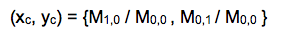
\includegraphics{images/Moments/centroid.png}
\caption{Centroid}
\end{figure}

where

\begin{figure}[htbp]
\centering
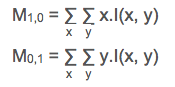
\includegraphics{images/Moments/m10m01.png}
\caption{}
\end{figure}

\textbf{Central moments}

Central moments are derived by reducing the spatial moments with
centroid. They are computed in a center referenced frame, in the
following manner-

\begin{figure}[htbp]
\centering
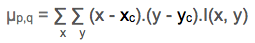
\includegraphics{images/Moments/central moments.png}
\caption{Central Moments}
\end{figure}

However, a disadvantage of spatial and central moments is that they are
dependant on the size of the object. So scaling is required. Area of the
object is generally used as a scaling factor. So, central normalized
moments are obtained by dividing the central moments with powers of
area.

\begin{figure}[htbp]
\centering
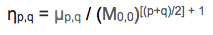
\includegraphics{images/Moments/central normalized moments.png}
\caption{Central Normalized Moments}
\end{figure}
\pagebreak
\textbf{Hu Moments} \\

Normalized moments are invariant to object size. However, they are
affected by the orientation of the image. To overcome this, we can use
Hu moments. Hu moments are invariant to translation, scaling and
rotation.

\begin{figure}[htbp]
\centering
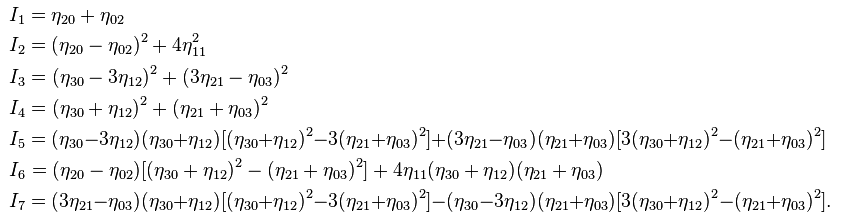
\includegraphics{images/Moments/hu.png}
\caption{Hu Moments}
\end{figure}

\subsection{Applications}\label{applications}

\begin{itemize}
\tightlist
\item
  Moments can be used to extract properties of an image.
\item
  They are used in pattern recognition.
\item
  Object identification also uses moments.
\item
  Image analysis is done using moments.
\end{itemize}

\section{Code}\label{code}

\subsection{Moments}\label{moments}

The main function we use to find moments is-

\begin{Shaded}
\begin{Highlighting}[]
    \NormalTok{cv2.moments(array[, binaryImage])}
\end{Highlighting}
\end{Shaded}

where

\begin{itemize}
	\item \textbf{array} : Raster image (single-channel, 8-bit or floating-point 2D array) or an array ( 1 times N or  N times 1 ) of 2D points (Point or Point2f ).

	\item \textbf{binaryImage} : If it is true, all non-zero image pixels are treated as 1’s. The parameter is used for images only.
\end{itemize}

\subsection{Hu Moments}\label{hu-moments}

The main function we use to find moments is-

\begin{Shaded}
\begin{Highlighting}[]
    \NormalTok{cv2.HuMoments(m[, hu])}
\end{Highlighting}
\end{Shaded}

where

\begin{verbatim}
m : Input moments.

hu : Output Hu invariants.
\end{verbatim}

Now, let us have a look at the code.

\begin{Shaded}
\begin{Highlighting}[]
\CommentTok{# Imports}
\ImportTok{import} \NormalTok{cv2}

\CommentTok{# Read image}
\NormalTok{img }\OperatorTok{=} \NormalTok{cv2.imread(}\StringTok{"images/example/example.jpg"}\NormalTok{)}

\CommentTok{# Convert to grayscale and apply thresholding}
\NormalTok{gray }\OperatorTok{=} \NormalTok{cv2.cvtColor(img, cv2.COLOR_BGR2GRAY)}
\NormalTok{ret, th }\OperatorTok{=} \NormalTok{cv2.threshold(gray, }\DecValTok{127}\NormalTok{, }\DecValTok{255}\NormalTok{, cv2.THRESH_BINARY)}

\CommentTok{# Find moments}
\NormalTok{M }\OperatorTok{=} \NormalTok{cv2.moments(th, }\VariableTok{True}\NormalTok{) }\CommentTok{#Second parameter is true as th is a binary image}

\BuiltInTok{print} \NormalTok{M}

\CommentTok{# Find Hu invariant moments}
\NormalTok{Hu }\OperatorTok{=} \NormalTok{cv2.HuMoments(M)}

\BuiltInTok{print} \NormalTok{Hu}
\end{Highlighting}
\end{Shaded}
\pagebreak
Consider the following image.

\begin{figure}[htbp]
\centering
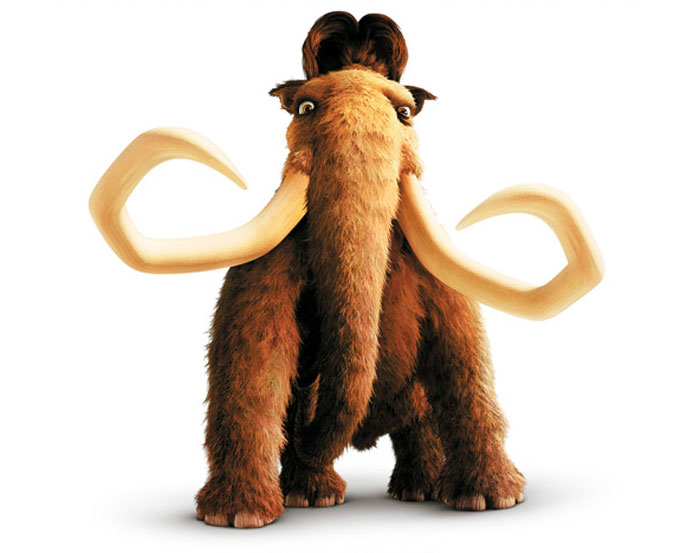
\includegraphics[width=6cm]{images/Moments/example.jpg}
\caption{Sample Image}
\end{figure}

When we find moments using cv2.moments(), we get this result-

\begin{figure}[htbp]
\centering
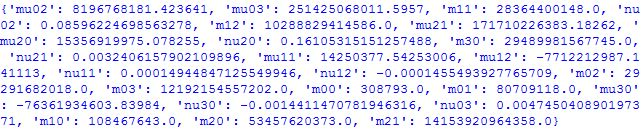
\includegraphics{images/Moments/result moments.JPG}
\caption{Output of moments}
\end{figure}

The Hu moments calculated will look like this-

\begin{figure}[htbp]
\centering
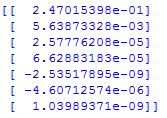
\includegraphics{images/Moments/result hu.JPG}
\caption{Output of Hu Moments}
\end{figure}
\pagebreak
\section{Resources}\label{resources}

\begin{itemize}
\tightlist
\item
  http://breckon.eu/toby/teaching/dip/opencv/SimpleImageAnalysisbyMoments.pdf
\item
  https://en.wikipedia.org/wiki/Image\_moment
\item
  http://docs.opencv.org/modules/imgproc/doc/structural\_analysis\_and\_shape\_descriptors.html
\item
  http://homepages.inf.ed.ac.uk/rbf/CVonline/LOCAL\_COPIES/SHUTLER3/node8.html
\item
  http://opencv-python-tutroals.readthedocs.org/en/latest/py\_tutorials/py\_imgproc/py\_contours/py\_contour\_features/py\_contour\_features.html\#contour-features
\end{itemize}

\end{document}
